\section{Polynomial-Time Reduction}

In Lecture~39, we designed an algorithm to solve the maximum matching problem on bipartite graphs
by \emph{transforming} it into a maximum-flow problem. This algorithm calls once a
solver for the maximum-flow problem~(in step 2), and it also builds the network~(in step 1)
and fetch the matching by processing the maximum-flow~(in step 3). This is a typical
example of so-called \emph{polynomial-time reduction}.
Such {reduction} is extremely useful---not only in solving new problems by using existing algorithms,
but also in proving that a problem is hard. Below we first formally define it.

\begin{definition}[Polynomial-Time Reduction]
Let $X$ and $Y$ be two problems.
If there exists an algorithm for $X$ which
calls a polynomial number of an algorithm for $Y$
and uses polynomial number of extra computational steps,
then we say $X$ is polynomial-time reducible to $Y$, denoted as $X \le_p Y$.
\end{definition}

In short, problem $X$ is polynomial-time reducible to problem $Y$ means ``we can design an algorithm for $X$ using an algorithm for $Y$''.
Of course, in this algorithm for $X$ the number of calls of a solver for $Y$ is limited to polynomial, and this algorithm for $X$
can have extra procedures, but these again need to run in polynomial-time.

Our algorithm for solving the maximum matching problem on bipartite graphs is such an example:
in that algorithm, we called once a solver for the maximum-flow problem; and the steps 1 and 3
takes polynomial-time. Therefore, we have (maximum-matching-problem-on-bipartite-graph) $\le_p$ (maximum-flow-problem).

Note that, above definition of polynomial-time reduction does \emph{not} require that
the algorithm for $Y$ runs in polynomial-time. It does not matter whether or not $Y$ can
be solved in polynomial-time. But, \emph{if} the solver for $Y$ runs in polynomial-time,
then the resulting algorithm for $X$ runs in polynomial-time as well, because 
a polynomial number of calls of an algorithm runs in polynomial-time also takes polynomial-time.
Formally,
\begin{fact}
If $X\le_p Y$ and $Y$ can be solved in polynomial-time, then $X$ can be solved in polynomial-time.
\end{fact}

\subsection*{Decision Problems}

A \emph{decision problem} refers to a problem with a \emph{binary} output, i.e., an algorithm
for this problem answers ``yes'' or ``no''.
For example, the 3SAT problem, which asks if a set of given clauses can be satisfied, is a decision problem.
Many of the problems we have seen in this course are \emph{optimization problems}. For examples, the maximum-flow problems
asks a flow, which is a function that assigns a number to each edge, of a given network, such that its value is maximized;
the (minimum) vertex cover problem asks a vertex cover, which is a subset of vertices, of a given undirected graph, 
such that its cardinality is minimized. These optimization problems are not decision problems.

Usually we can define a \emph{decision-version} of an optimization problem. Let's try it for the vertex cover problem;
its decision-version can be defined as follows: given an undirected graph $G = (V, E)$ and an integer $k\ge 0$,
decide if there exists a vertex cover $V_1$ of $G$ such that $|V_1| \le k$. In other words, the problem asks if the
given $k$ is an upper-bound of the cardinality of the minimum vertex cover of the given undirected graph.
%Note that its input includes both an undirected graph and an integer.

We use $VC(G)$ to refer to the (optimization-version) of the vertex-cover problem, and use $VC(G, k)$ to refer to
above decision-version of the vertex-cover problem. What's the ralationship between them? Here by ``relationship''
we specifically ask if one problem is polynomial-time reducible to the other. Intuitively, the decision-version
is ``easier'' than the optimization-version, and we can easily use an algorithm for the optimization-version
to solver the decision-version.
\begin{fact}
$VC(G, k)\le_p VC(G)$.
\end{fact}
\emph{Proof.} To prove that $VC(G,k)$ is polynomial-time reducible to $VC(G)$, by definition, 
we need to design an algorithm for $VC(G, k)$, in which we can assume and use, up to polynomial number of calls,
a solver for $VC(G)$. Here is such an algorithm:

\begin{minipage}{0.8\textwidth}
	\aaA {4}{algorithm-for-$VC(G, k)$}\xxx
	\aab {call the solver for $VC(G)$ to get the minimum vertex cover of $G$: $V_1^* \leftarrow $ solver-for-$VC(G)$;}\xxx
	\aab {if $|V_1^*| \le k$: return ``yes'';}\xxx
	\aab {else: return ``no'';}\xxx
	\aaa {end;}\xxx
\end{minipage}

Clearly, this algorithm for $VC(G, k)$ is correct; it calls once (and hence polynomial number)
a solver for $VC(G)$, and the additional procedure~(which just compares $|V_1^*|$ with the given $k$)
runs in constant time~(and hence in polynomial-time). This proves that $VC(G, k)\le_p VC(G)$. \qed

How about the other side? Is $VC(G)$ polynomial-time reducible to $VC(G, k)$? It's not obvious but 
this is true as well. Formally,
\begin{fact}
$VC(G)\le_p VC(G, k)$.
\end{fact}
\emph{Proof.}  Again we need to design an algorithm for $VC(G)$ using a solver for $VC(G, k)$.
Recall that a solver for the decision-version tells if a given $k$ is an upper-bound of the
cardinality of the minimum vertex cover of $G$. 
Therefore we can calculate the \emph{cardinality} of the minimum vertex cover of $G$,
by testing all possible sizes of a subset of vertices in \emph{increasing} order,
   i.e., $0, 1, 2, \cdots, |V|$;
the first achievable value is the \emph{cardinality} of the minimum vertex cover.

\begin{minipage}{0.8\textwidth}
	\aaA {5}{algorithm-for-cardinality-$VC(G)$}\xxx
	\aaB {3}{for $k = 0 \to |V|$}\xxx
	\aac {call the solver for the decision-version to test the given $G$ and this $k$: $B \leftarrow $ solver-for-$VC(G, k)$;}\xxx
	\aac {if $B$ = ``yes'': return $k$;}\xxx
	\aab {end for;}\xxx
	\aaa {end;}\xxx
\end{minipage}

This algorithm finds the cardinality of the minimum vertex cover of $G$; we denote it by $k^*$.
How can we then find the actual vertex cover? Here is one strategy:
we determine a single vertex that must be in one minimum vertex cover; if
this can be done, we can then
include that vertex (to the minimum vertex cover) and resolve the ``remaining part'' of the graph recursively.
The core procedure is therefore to determine if a vertex is in one minimum vertex cover,
which can be solved based on this fact: let $v\in V$ be a vertex; 
there exists a minimum vertex cover that includes $v$
if and only if the ``remaining-graph'' $G_{-v}$, defined as the graph by removing $v$ and adjacent edges of $v$ from $G$, can
be covered by $(k^* - 1)$ vertices. 
See Figure~\ref{fig:cover}.  
Note that, the solver for the decision-version can be used to answer 
whether any graph, in this case the remaining graph $G_{-v}$, can be covered by $(k^* - 1)$ vertices. 

\begin{figure}[h]
\centering{

\tikzset{every picture/.style={line width=0.75pt}} %set default line width to 0.75pt        

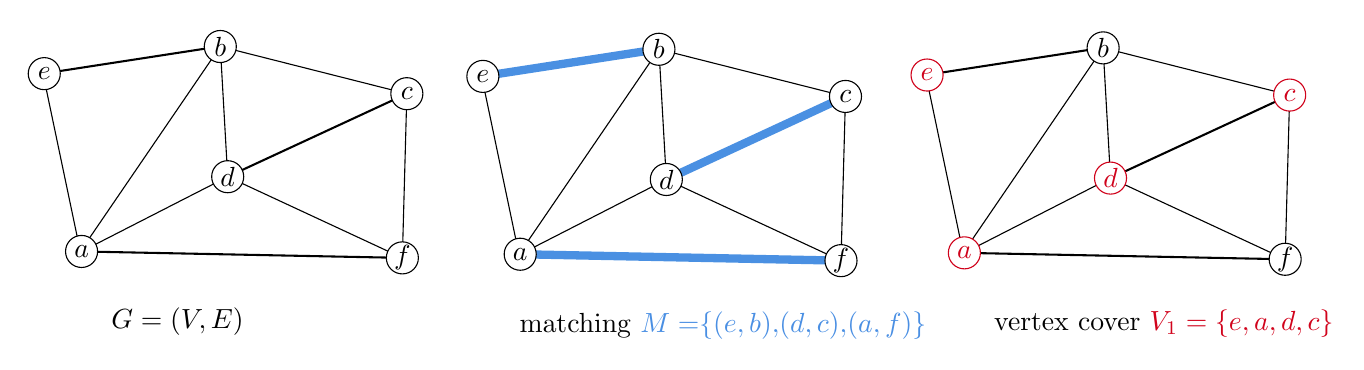
\begin{tikzpicture}[x=0.5pt,y=0.5pt,yscale=-1,xscale=1]
%uncomment if require: \path (0,237); %set diagram left start at 0, and has height of 237

%Straight Lines [id:da7485926733039977] 
\draw    (144.6,14.97) -- (43.43,163.09) ;
%Straight Lines [id:da4575120980127291] 
\draw [color={rgb, 255:red, 0; green, 0; blue, 0 }  ,draw opacity=1 ][line width=0.75]    (16.46,34.58) -- (143.69,14.97) ;
%Straight Lines [id:da9165715401778428] 
\draw    (16.46,34.58) -- (43.43,163.09) ;
%Straight Lines [id:da994182434786223] 
\draw [color={rgb, 255:red, 0; green, 0; blue, 0 }  ,draw opacity=1 ][line width=0.75]    (44.34,163.09) -- (276.17,167.73) ;
%Straight Lines [id:da9750224919648968] 
\draw    (149.95,109.07) -- (276.17,167.73) ;
%Straight Lines [id:da24348552449211425] 
\draw    (144.6,14.97) -- (149.95,109.07) ;
%Straight Lines [id:da16705340438790406] 
\draw    (144.6,14.97) -- (279.42,49.07) ;
%Straight Lines [id:da08663700279220432] 
\draw    (279.42,49.07) -- (276.17,167.73) ;
%Straight Lines [id:da16511775802360662] 
\draw [color={rgb, 255:red, 0; green, 0; blue, 0 }  ,draw opacity=1 ][line width=0.75]    (279.42,49.07) -- (149.95,109.07) ;
%Straight Lines [id:da4151454155794566] 
\draw    (149.95,109.07) -- (44.34,163.09) ;
%Shape: Ellipse [id:dp9133580928774087] 
\draw  [fill={rgb, 255:red, 255; green, 255; blue, 255 }  ,fill opacity=1 ] (5.79,34.58) .. controls (5.79,28.18) and (10.97,23) .. (17.37,23) .. controls (23.76,23) and (28.95,28.18) .. (28.95,34.58) .. controls (28.95,40.97) and (23.76,46.16) .. (17.37,46.16) .. controls (10.97,46.16) and (5.79,40.97) .. (5.79,34.58) -- cycle ;
%Shape: Ellipse [id:dp4005957609675306] 
\draw  [fill={rgb, 255:red, 255; green, 255; blue, 255 }  ,fill opacity=1 ] (133.02,14.97) .. controls (133.02,8.57) and (138.2,3.39) .. (144.6,3.39) .. controls (151,3.39) and (156.18,8.57) .. (156.18,14.97) .. controls (156.18,21.36) and (151,26.55) .. (144.6,26.55) .. controls (138.2,26.55) and (133.02,21.36) .. (133.02,14.97) -- cycle ;
%Shape: Ellipse [id:dp49214617921702164] 
\draw  [fill={rgb, 255:red, 255; green, 255; blue, 255 }  ,fill opacity=1 ] (267.84,49.07) .. controls (267.84,42.67) and (273.02,37.49) .. (279.42,37.49) .. controls (285.82,37.49) and (291,42.67) .. (291,49.07) .. controls (291,55.46) and (285.82,60.65) .. (279.42,60.65) .. controls (273.02,60.65) and (267.84,55.46) .. (267.84,49.07) -- cycle ;
%Shape: Ellipse [id:dp8440754424343925] 
\draw  [fill={rgb, 255:red, 255; green, 255; blue, 255 }  ,fill opacity=1 ] (138.37,109.07) .. controls (138.37,102.68) and (143.55,97.49) .. (149.95,97.49) .. controls (156.34,97.49) and (161.53,102.68) .. (161.53,109.07) .. controls (161.53,115.47) and (156.34,120.65) .. (149.95,120.65) .. controls (143.55,120.65) and (138.37,115.47) .. (138.37,109.07) -- cycle ;
%Shape: Ellipse [id:dp20660183368429152] 
\draw  [fill={rgb, 255:red, 255; green, 255; blue, 255 }  ,fill opacity=1 ] (32.76,163.09) .. controls (32.76,156.7) and (37.94,151.51) .. (44.34,151.51) .. controls (50.73,151.51) and (55.92,156.7) .. (55.92,163.09) .. controls (55.92,169.49) and (50.73,174.67) .. (44.34,174.67) .. controls (37.94,174.67) and (32.76,169.49) .. (32.76,163.09) -- cycle ;
%Shape: Ellipse [id:dp4098192910838151] 
\draw  [fill={rgb, 255:red, 255; green, 255; blue, 255 }  ,fill opacity=1 ] (264.59,167.73) .. controls (264.59,161.33) and (269.77,156.15) .. (276.17,156.15) .. controls (282.56,156.15) and (287.75,161.33) .. (287.75,167.73) .. controls (287.75,174.13) and (282.56,179.31) .. (276.17,179.31) .. controls (269.77,179.31) and (264.59,174.13) .. (264.59,167.73) -- cycle ;
%Straight Lines [id:da6233481480623783] 
\draw    (461.6,16.97) -- (360.43,165.09) ;
%Straight Lines [id:da9901942575404544] 
\draw [color={rgb, 255:red, 74; green, 144; blue, 226 }  ,draw opacity=1 ][line width=3]    (333.46,36.58) -- (460.69,16.97) ;
%Straight Lines [id:da3790939323014558] 
\draw    (333.46,36.58) -- (360.43,165.09) ;
%Straight Lines [id:da42115713644274366] 
\draw [color={rgb, 255:red, 74; green, 144; blue, 226 }  ,draw opacity=1 ][line width=3]    (361.34,165.09) -- (593.17,169.73) ;
%Straight Lines [id:da8702690824311631] 
\draw    (466.95,111.07) -- (593.17,169.73) ;
%Straight Lines [id:da34939805445985417] 
\draw    (461.6,16.97) -- (466.95,111.07) ;
%Straight Lines [id:da04544520748950576] 
\draw    (461.6,16.97) -- (596.42,51.07) ;
%Straight Lines [id:da5361594760285122] 
\draw    (596.42,51.07) -- (593.17,169.73) ;
%Straight Lines [id:da10465085418843478] 
\draw [color={rgb, 255:red, 74; green, 144; blue, 226 }  ,draw opacity=1 ][line width=3]    (596.42,51.07) -- (466.95,111.07) ;
%Straight Lines [id:da555393377892622] 
\draw    (466.95,111.07) -- (361.34,165.09) ;
%Shape: Ellipse [id:dp39324544068995604] 
\draw  [fill={rgb, 255:red, 255; green, 255; blue, 255 }  ,fill opacity=1 ] (322.79,36.58) .. controls (322.79,30.18) and (327.97,25) .. (334.37,25) .. controls (340.76,25) and (345.95,30.18) .. (345.95,36.58) .. controls (345.95,42.97) and (340.76,48.16) .. (334.37,48.16) .. controls (327.97,48.16) and (322.79,42.97) .. (322.79,36.58) -- cycle ;
%Shape: Ellipse [id:dp8663152391911655] 
\draw  [fill={rgb, 255:red, 255; green, 255; blue, 255 }  ,fill opacity=1 ] (450.02,16.97) .. controls (450.02,10.57) and (455.2,5.39) .. (461.6,5.39) .. controls (468,5.39) and (473.18,10.57) .. (473.18,16.97) .. controls (473.18,23.36) and (468,28.55) .. (461.6,28.55) .. controls (455.2,28.55) and (450.02,23.36) .. (450.02,16.97) -- cycle ;
%Shape: Ellipse [id:dp9564869279164044] 
\draw  [fill={rgb, 255:red, 255; green, 255; blue, 255 }  ,fill opacity=1 ] (584.84,51.07) .. controls (584.84,44.67) and (590.02,39.49) .. (596.42,39.49) .. controls (602.82,39.49) and (608,44.67) .. (608,51.07) .. controls (608,57.46) and (602.82,62.65) .. (596.42,62.65) .. controls (590.02,62.65) and (584.84,57.46) .. (584.84,51.07) -- cycle ;
%Shape: Ellipse [id:dp14244956479013948] 
\draw  [fill={rgb, 255:red, 255; green, 255; blue, 255 }  ,fill opacity=1 ] (455.37,111.07) .. controls (455.37,104.68) and (460.55,99.49) .. (466.95,99.49) .. controls (473.34,99.49) and (478.53,104.68) .. (478.53,111.07) .. controls (478.53,117.47) and (473.34,122.65) .. (466.95,122.65) .. controls (460.55,122.65) and (455.37,117.47) .. (455.37,111.07) -- cycle ;
%Shape: Ellipse [id:dp3916752397044988] 
\draw  [fill={rgb, 255:red, 255; green, 255; blue, 255 }  ,fill opacity=1 ] (349.76,165.09) .. controls (349.76,158.7) and (354.94,153.51) .. (361.34,153.51) .. controls (367.73,153.51) and (372.92,158.7) .. (372.92,165.09) .. controls (372.92,171.49) and (367.73,176.67) .. (361.34,176.67) .. controls (354.94,176.67) and (349.76,171.49) .. (349.76,165.09) -- cycle ;
%Shape: Ellipse [id:dp6775141746120102] 
\draw  [fill={rgb, 255:red, 255; green, 255; blue, 255 }  ,fill opacity=1 ] (581.59,169.73) .. controls (581.59,163.33) and (586.77,158.15) .. (593.17,158.15) .. controls (599.56,158.15) and (604.75,163.33) .. (604.75,169.73) .. controls (604.75,176.13) and (599.56,181.31) .. (593.17,181.31) .. controls (586.77,181.31) and (581.59,176.13) .. (581.59,169.73) -- cycle ;
%Straight Lines [id:da991028078692109] 
\draw    (782.6,15.97) -- (681.43,164.09) ;
%Straight Lines [id:da8020042074548936] 
\draw [color={rgb, 255:red, 0; green, 0; blue, 0 }  ,draw opacity=1 ][line width=0.75]    (654.46,35.58) -- (781.69,15.97) ;
%Straight Lines [id:da5410354625843318] 
\draw    (654.46,35.58) -- (681.43,164.09) ;
%Straight Lines [id:da1284005435452643] 
\draw [color={rgb, 255:red, 0; green, 0; blue, 0 }  ,draw opacity=1 ][line width=0.75]    (682.34,164.09) -- (914.17,168.73) ;
%Straight Lines [id:da4841445577516499] 
\draw    (787.95,110.07) -- (914.17,168.73) ;
%Straight Lines [id:da3189236797568633] 
\draw    (782.6,15.97) -- (787.95,110.07) ;
%Straight Lines [id:da24633327282247075] 
\draw    (782.6,15.97) -- (917.42,50.07) ;
%Straight Lines [id:da666695835406161] 
\draw    (917.42,50.07) -- (914.17,168.73) ;
%Straight Lines [id:da31804257401559455] 
\draw [color={rgb, 255:red, 0; green, 0; blue, 0 }  ,draw opacity=1 ][line width=0.75]    (917.42,50.07) -- (787.95,110.07) ;
%Straight Lines [id:da6699316806179542] 
\draw    (787.95,110.07) -- (682.34,164.09) ;
%Shape: Ellipse [id:dp818344887208882] 
\draw  [color={rgb, 255:red, 208; green, 2; blue, 27 }  ,draw opacity=1 ][fill={rgb, 255:red, 255; green, 255; blue, 255 }  ,fill opacity=1 ] (643.79,35.58) .. controls (643.79,29.18) and (648.97,24) .. (655.37,24) .. controls (661.76,24) and (666.95,29.18) .. (666.95,35.58) .. controls (666.95,41.97) and (661.76,47.16) .. (655.37,47.16) .. controls (648.97,47.16) and (643.79,41.97) .. (643.79,35.58) -- cycle ;
%Shape: Ellipse [id:dp5629283730413089] 
\draw  [fill={rgb, 255:red, 255; green, 255; blue, 255 }  ,fill opacity=1 ] (771.02,15.97) .. controls (771.02,9.57) and (776.2,4.39) .. (782.6,4.39) .. controls (789,4.39) and (794.18,9.57) .. (794.18,15.97) .. controls (794.18,22.36) and (789,27.55) .. (782.6,27.55) .. controls (776.2,27.55) and (771.02,22.36) .. (771.02,15.97) -- cycle ;
%Shape: Ellipse [id:dp21443256600205352] 
\draw  [color={rgb, 255:red, 208; green, 2; blue, 27 }  ,draw opacity=1 ][fill={rgb, 255:red, 255; green, 255; blue, 255 }  ,fill opacity=1 ] (905.84,50.07) .. controls (905.84,43.67) and (911.02,38.49) .. (917.42,38.49) .. controls (923.82,38.49) and (929,43.67) .. (929,50.07) .. controls (929,56.46) and (923.82,61.65) .. (917.42,61.65) .. controls (911.02,61.65) and (905.84,56.46) .. (905.84,50.07) -- cycle ;
%Shape: Ellipse [id:dp17023173827913307] 
\draw  [color={rgb, 255:red, 208; green, 2; blue, 27 }  ,draw opacity=1 ][fill={rgb, 255:red, 255; green, 255; blue, 255 }  ,fill opacity=1 ] (776.37,110.07) .. controls (776.37,103.68) and (781.55,98.49) .. (787.95,98.49) .. controls (794.34,98.49) and (799.53,103.68) .. (799.53,110.07) .. controls (799.53,116.47) and (794.34,121.65) .. (787.95,121.65) .. controls (781.55,121.65) and (776.37,116.47) .. (776.37,110.07) -- cycle ;
%Shape: Ellipse [id:dp21431691922786544] 
\draw  [color={rgb, 255:red, 208; green, 2; blue, 27 }  ,draw opacity=1 ][fill={rgb, 255:red, 255; green, 255; blue, 255 }  ,fill opacity=1 ] (670.76,164.09) .. controls (670.76,157.7) and (675.94,152.51) .. (682.34,152.51) .. controls (688.73,152.51) and (693.92,157.7) .. (693.92,164.09) .. controls (693.92,170.49) and (688.73,175.67) .. (682.34,175.67) .. controls (675.94,175.67) and (670.76,170.49) .. (670.76,164.09) -- cycle ;
%Shape: Ellipse [id:dp6777828112816564] 
\draw  [fill={rgb, 255:red, 255; green, 255; blue, 255 }  ,fill opacity=1 ] (902.59,168.73) .. controls (902.59,162.33) and (907.77,157.15) .. (914.17,157.15) .. controls (920.56,157.15) and (925.75,162.33) .. (925.75,168.73) .. controls (925.75,175.13) and (920.56,180.31) .. (914.17,180.31) .. controls (907.77,180.31) and (902.59,175.13) .. (902.59,168.73) -- cycle ;

% Text Node
\draw (17.37,34.58) node   [align=left] {$\displaystyle e$};
% Text Node
\draw (144.6,14.97) node   [align=left] {$\displaystyle b$};
% Text Node
\draw (279.42,49.07) node   [align=left] {$\displaystyle c$};
% Text Node
\draw (149.95,109.07) node   [align=left] {$\displaystyle d$};
% Text Node
\draw (44.34,163.09) node   [align=left] {$\displaystyle a$};
% Text Node
\draw (276.17,167.73) node   [align=left] {$\displaystyle f$};
% Text Node
\draw (64,202) node [anchor=north west][inner sep=0.75pt]   [align=left] {$\displaystyle G=( V,E)$};
% Text Node
\draw (334.37,36.58) node   [align=left] {$\displaystyle e$};
% Text Node
\draw (461.6,16.97) node   [align=left] {$\displaystyle b$};
% Text Node
\draw (596.42,51.07) node   [align=left] {$\displaystyle c$};
% Text Node
\draw (466.95,111.07) node   [align=left] {$\displaystyle d$};
% Text Node
\draw (361.34,165.09) node   [align=left] {$\displaystyle a$};
% Text Node
\draw (593.17,169.73) node   [align=left] {$\displaystyle f$};
% Text Node
\draw (359,205) node [anchor=north west][inner sep=0.75pt]   [align=left] {matching $\displaystyle \textcolor[rgb]{0.29,0.56,0.89}{M=}\textcolor[rgb]{0.29,0.56,0.89}{\{}\textcolor[rgb]{0.29,0.56,0.89}{(}\textcolor[rgb]{0.29,0.56,0.89}{e,b}\textcolor[rgb]{0.29,0.56,0.89}{)}\textcolor[rgb]{0.29,0.56,0.89}{,}\textcolor[rgb]{0.29,0.56,0.89}{(}\textcolor[rgb]{0.29,0.56,0.89}{d,c}\textcolor[rgb]{0.29,0.56,0.89}{)}\textcolor[rgb]{0.29,0.56,0.89}{,}\textcolor[rgb]{0.29,0.56,0.89}{(}\textcolor[rgb]{0.29,0.56,0.89}{a,f}\textcolor[rgb]{0.29,0.56,0.89}{)}\textcolor[rgb]{0.29,0.56,0.89}{\}}$};
% Text Node
\draw (655.37,35.58) node  [color={rgb, 255:red, 208; green, 2; blue, 27 }  ,opacity=1 ] [align=left] {$\displaystyle e$};
% Text Node
\draw (782.6,15.97) node   [align=left] {$\displaystyle b$};
% Text Node
\draw (917.42,50.07) node  [color={rgb, 255:red, 208; green, 2; blue, 27 }  ,opacity=1 ] [align=left] {$\displaystyle c$};
% Text Node
\draw (787.95,110.07) node  [color={rgb, 255:red, 208; green, 2; blue, 27 }  ,opacity=1 ] [align=left] {$\displaystyle d$};
% Text Node
\draw (682.34,164.09) node  [color={rgb, 255:red, 208; green, 2; blue, 27 }  ,opacity=1 ] [align=left] {$\displaystyle a$};
% Text Node
\draw (914.17,168.73) node   [align=left] {$\displaystyle f$};
% Text Node
\draw (702,203) node [anchor=north west][inner sep=0.75pt]   [align=left] {vertex cover $\displaystyle \textcolor[rgb]{0.82,0.01,0.11}{V_{1} =\{e,a,d,c\}}$};


\end{tikzpicture}

}
\caption{Illustrating that a vertex $v$ is in one minimum vertex cover if and only if
$G_{-v}$ can be covered by $k^* - 1$ vertices, where $k^*$ is defined as the cardinality of any minimum vertex cover of $G$.}
%\emph{Proof.} If $G_{-v}$ can be covered by $k^* - 1$ vertices, i.e., there exists a vertex cover $V_2^*$
%for $G_{-v}$ with $|V_2^*| = k^* - 1$, then $V_2^* \cup \{v\}$ is a vertex cover of $G$,
%and its cardinality is $k^*$. This shows that that $V_2^* \cup \{v\}$ is a minimum vertex cover of $G$ 
%as its size is minimized, and it includes $v$. On the other hand, 
\label{fig:cover}
\end{figure}


\begin{minipage}{0.8\textwidth}
	\aaA {9}{algorithm-for-$VC(G)$}\xxx
	\aab {$k^* \leftarrow $ algorithm-for-cardinality-$VC(G)$;}\xxx
	\aaB {4}{for each $v \in V$}\xxx
	\aac {build the remaining graph $G_{-v}$ by removing $v$ and its adjacent edges from $G$;}\xxx
	\aac {call the solver for the decision-version to test $G_{-v}$ and $k^*-1$: $B \leftarrow $ solver-for-$VC(G_{-v}, k^*-1)$;}\xxx
	\aac {if $B$ = ``yes'': save this $v$ as $u$ and break the for-loop;}\xxx
	\aab {end for;}\xxx
	\aab {resolve the remaining graph $G_{-u}$: $V_2^* \leftarrow $ algorithm-for-$VC(G_{-u})$;}\xxx
	\aab {return $\{u\}\cup V_2^*$;}\xxx
	\aaa {end;}\xxx
\end{minipage}

The complete algorithm for the optimization version is given above.
Note that this algorithm is a recursive algorithm, and we define
that algorithm-for-$VC(G)$ returns the actual minimum vertex cover of $G$.
What's its running time? Note that it calls itself once, i.e., 
algorithm-for-$VC(G_{-u})$, and the number of vertices in this call
is reduced by 1. Besides, it calls algorithm-for-cardinality-$VC(G)$,
which requires $|V|$ calls to solver-for-$VC(G, k)$,
and the for-loop requires another $|V|$ calls to solver-for-$VC(G, k)$.
Combined, its running time $T(n)$, where $n = |V|$, can be written
as $T(n) = T(n-1) + 2n\cdot solver(G,k)$, where $solver(G,k)$ represents
the running time of calling solver-for-$VC(G, k)$ once.
Solving this recurrence gives $T(n) = O(n^2)\cdot solver(G,k)$.

This proves $VC(G) \le_p VC(G,k)$, as we designed an algorithm
for $VC(G)$, which uses $O(n^2)$, a polynomial number, of calls
to a solver for $VC(G, k)$. \qed

These two facts show that the decision-version and the optimization-version
of the vertex cover problem are essentially equivalent, in terms of that they are mutually polynomial-time reducible.
Such conclusion are true for most optimization problems.
This is useful in simplying the hierarchy of problems: now we can solely focus on decision problems, as they are simpler~(the output is just a single bit),
while also captures the hardness of the optimization version~(equivalent in terms of polynomial-time reduction).

\subsection*{P and NP}

In complexity theory, ``P'' is defined as the set of decision problems that are \emph{polynomial-time solvable}, 
and ``NP'' is defined as the set of decision problems that are \emph{polynomial-time verifiable}, 
Polynomial-time solvable means that one can design a polynomial-time algorithm to \emph{solve} the problem.
Polynomial-time verifiable means that one can design a polynomial-time algorithm to \emph{verify}
if a \emph{given} solution~(also called a \emph{certificate}) is correct,  
and such certificate must exist for ``yes''-instances.
They are formally defined below.

%formally stated below. 

\begin{definition}[P]
Let $X$ be a decision problem. We say $X\in \textrm{P}$ if there exists a polynomial-time algorithm $A$~(we call $A$ as a \emph{solver}), such that,\\
	(1), solver $A$ takes an instance $x$ of $X$ as input, and \\
	(2), for every instance $x$ of problem $X$: \\
	\hspace*{0.2cm} if the ground-truth of $x$ is ``yes'', then $A(x)$ returns ``yes'';\\
	\hspace*{0.2cm} if the ground-truth of $x$ is ``no'', then $A(x)$ returns ``no''.
\end{definition}

In above definition, condition (1) means that algorithm $A$ is \emph{for solving} problem $X$;
condition (2) means that algorithm $A$ is correct: every instance has a ``ground-truth'' answer, and
algorithm $A$ always finds it.

\begin{definition}[NP]
Let $X$ be a decision problem. We say $X\in \textrm{NP}$ if there exists a polynomial-time algorithm $A$~(we call $A$ as a \emph{verifier}), such that,\\
	(1), verifier $A$ takes an instance $x$ of $X$ \emph{and} a polynomial-length certificate $c$ as input, and \\
	(2), for every instance $x$ of problem $X$: \\
	\hspace*{0.2cm} if the ground-truth of $x$ is ``yes'', then there must exist a certificate $c$ such that $A(x,c)$ returns ``yes'';\\
	\hspace*{0.2cm} if the ground-truth of $x$ is ``no'', then for any polynomial-length certificate $c$, $A(x,c)$ always returns ``no''.
\end{definition}

In above definition, condition (1) means that algorithm $A$ is for verifying if the (given) certificate is the correct solution of the (given) instance;
condition (2) means there exists (polynomial-length) certificate
for every ``yes''-instnace but not for any ``no''-instance, and they can be correctly verified by algorithm $A$.
Notice that, \emph{how to find} such correct certificate is not the job of algorithm $A$.
When we use this definition to show that a problem is in NP, we just need to argue that
such certificate \emph{exists}, we don't need to design algorithms to find it out.
We give two examples below.

\begin{fact}
3SAT problem is in NP.
\end{fact}
\emph{Proof.} By definition, to prove 3SAT is in NP, we need to design an
algorithm~(i.e., the verifier $A$), and show that it satisfies the two
conditions. For 3SAT, the certificate is an assignment for all variables,
which can be represented as a binary vector. The verifier, given below, will check
if the given binary vector is in correct length, and if it satisfies all clauses,
and these can be done in polynomial-time.

\begin{minipage}{0.8\textwidth}
	\aaA {4}{verifier~$(x, c)$}\xxx
	\aab {verify that the length of $c$ equals to the number of variables in instance $x$: if not, return ``no'';}\xxx
	\aab {verify that every clause in instance $x$ is true when $x_i$ is assigned with $c[i]$: if not, return ``no'';}\xxx
	\aab {return ``yes'';}\xxx
	\aaa {end;}\xxx
\end{minipage}

Now we prove that above verifier satisfies the two conditions.
It clearly takes an instance and a certificate as input.
If $x$ is an ``yes''-instance, then it means $x$ is satisfiable, i.e.,
there exists an assignment that satisfies all clauses.
Clearly, once this assignment is passed to the verifier together with $x$,
the verifier will return ``yes''.
If $x$ is an ``no''-instance, then it means $x$ is not satisfiable, i.e.,
there does not exist an assignment that satisfies all clauses.
Hence, no matter which assignment is passed to the verifier with $x$,
the verifier always returns ``no''. Also, verifier $A$ runs in polynomial-time.
This proves that 3SAT is in NP.
\qed


\begin{fact}
The decision-version of vertex cover problem, i.e., $VC(G, k)$, is in NP.
\end{fact}

\emph{Proof.} Again we design an algorithm~(i.e., the verifier $A$), and show that it satisfies the two
conditions. For $VC(G, k)$, the certificate is a subset of vertices, which
can be represented as a vector.
The verifier, given below, will verify its size, and verify if it covers all edges.

\begin{minipage}{0.8\textwidth}
	\aaA {4}{verifier~$(x = (G, k), c)$}\xxx
	\aab {verify the size of $c$ is at most $k$: if not, return ``no'';}\xxx
	\aab {verify the vertices in $c$ can cover all edges of $G$: if not, return ``no'';}\xxx
	\aab {return ``yes'';}\xxx
	\aaa {end;}\xxx
\end{minipage}

Above verifier takes an instance and a certificate as input.
If $x = (G, k)$ is an ``yes''-instance, then it means there exists a subset of vertices $V_1$
with $|V_1| \le k$ and $V_1$ covers all edges in $G$.
Hence, once this $V_1$ is passed to the verifier together with $x$,
the verifier will return ``yes''.
If $x$ is an ``no''-instance, then it does not exist a subset with at most $k$ vertices
that covers all edges in $G$.
Hence, no matter which subset of vertices~(coded in $c$) is passed to the verifier with $x$,
the verifier always returns ``no''---either because it exceeds $k$ vertices,
or does not cover all edges.  Also, verifier $A$ runs in polynomial-time.
\qed

